\chapter{Topološka analiza podatkov}
Topološka analiza podatkov (TDA, ang. topological data analysis) je novejša veda, ki se je začela razvijati šele v zgodnjih letih tega tisočletja. Navdih za njen razvoj izhaja iz tega, da lahko s koncepti iz topologije (vede oblik) in geometrije (vede prostora in dimenzij)  razumemo strukturo kompleksnih podatkov kot tudi nekatere podrobne in specifične informacije o njih. Ta pristop nam pomaga vizualizirati in analizirati celotno strukturo in vzorce, ki se skrivajo v podatkih, ter je manj občutljiv na majhne spremembe ali šume. TDA nam ponuja ogromno metod za analizo podatkov, ki so običajno predstavljeni v obliki oblaka oz. množice točk (ang. point cloud).

V tem poglavju bomo obravnavali nekaj osnovnih pojmov TDA, ki nam bodo kasneje v pomoč za vizualizacijo nevronske mreže s pomočjo algoritma Mapper. Defnirali bomo simplicialne komplekse in predstavili različne načine konstrukcije na podatkovnih množicah. Podali bomo Izrek o živcu, ki je glava motivacija za uporabo metod topološke analize podatkov.



\section{Glavni koraki TDA}
Kljub temu, da dandanes obstaja že veliko metod z različnimi aplikacijami, jih večina sledi naslednjim korakom:
\begin{enumerate}
    \item Vhod predstavlja končna množica točk z določeno razdaljo ali merilom podobnosti, ki je lahko osnovana na metriki okoljskega prostora (kot je evklidska v $R^d$) ali na lastni metriki, izračunani iz matrike razdalj med pari. Ta metrika je pogosto vnaprej določena ali diktirana s strani specifične uporabe. Vendar pa je izbira prave metrike ključnega pomena za odkrivanje pomembnih topoloških in geometrijskih lastnosti podatkov.
    \item Nad podatki se ustvari kontinuirana struktura, običajno preprost kompleks ali serija takih kompleksov, znana kot filtracija, ki razkriva topologijo ali geometrijo podatkov. Ti kompleksi, ki so v bistvu razširitve grafov v višje dimenzije, pomagajo prikazati strukturo podatkov na različnih ravneh. Izziv je ustvariti strukture, ki ne le natančno odražajo strukturo podatkov, ampak jih je tudi mogoče učinkovito graditi in spreminjati.
    \item Iz teh struktur se izluščijo topološke ali geometrijske podrobnosti. To lahko vključuje rekonstrukcijo osnovne oblike podatkov, na primer s triangulacijo, kar olajša dostop do njenih značilnosti, ali ustvarjanje preprostih povzetkov, ki zahtevajo specializirane metode, kot je trajna homologija, za pridobivanje nekaterih informacij. Ključna naloga tukaj je dokazati uporabnost in zanesljivost teh informacij, še posebej, kako se obnesejo v primeru napak ali šuma v podatkih.
    \item Razkrite informacije o topologiji in geometriji podatkov nudijo nove vrste značilnosti in opisov. Te lahko izboljšajo naše razumevanje podatkov, zlasti preko vizualnih metod, ali pa se integrirajo z drugimi značilnostmi podatkov za širšo analizo in aplikacije strojnega učenja. Uporaba teh informacij za ustvarjanje prilagojenih modelov analize podatkov in strojnega učenja je ključni del izkoriščanja tega, kar ponujajo orodja TDA.
\end{enumerate}

\section{Simpleks}
V nadaljevanju bomo potrebovali pojem simplicialnih kompleksov, katerih osnovni gradniki so simpleksi, ki jih bomo opisali v tem razdelku. Pri tem bomo sledili \cite{Urbančič_2020} in  Intuitivno so $n$-simpleksi geometrijski objekti z $(n + 1)$ oglišči, ki ležijo v $n$-dimenzionalnem prostoru in jih ne moremo vstaviti v nižje dimenzionalni prostor. Za gradnjo $n$-simpleksa v $n$-dimenzionalnem prostoru potrebujemo $(n + 1)$ afino neodvisnih točk.
\begin{definicija}
    Množica točk $\{x_0, \dots, x_n\}$ v vektorskem prostoru $V$ je \textbf{afino neodvisna}, če je $\{x_1 - x_0, \dots, x_n - x_0\}$ linearno neodvisna.
\end{definicija}

Matematično lahko simplekse definiramo na naslednji način.
\begin{definicija}
Naj bo \(X = \{x_0, x_1, \dots, x_n\}\) poljubna družina afino neodvisnih točk v prostoru \(\mathbb{R}^d\) za nek \(n \geq d\). Konveksno ovojnico množice \(X\),
\[
C_n(X) = C_k(x_0, x_1, \dots, x_n) = \{\sum_{i=0}^n \alpha_i x_i : \forall \alpha_i \in [0, 1], \sum_{i=0}^n \alpha_i = 1\},
\]
imenujemo \(n\)-simpleks na množici \(X\).
\end{definicija}
Točke \(X\) imenujemo oglišča \(\sigma\), simplekse ki jih razpenjajo podmnožice \(X\) pa imenujemo lica \(\sigma\).
\begin{comment}
\begin{definicija}
    Za množico \(X = \{x_0, \dots, x_k\} \subseteq \mathbb{R}^d\), \(k + 1\) afino neodvisnih točk, je \(k\)-dimenzionalni simpleks \(\sigma = [x_0, \dots, x_k]\), ki ga razpenja \(X\) konveksna ogrinjača \(X\). \\
Točke \(X\) imenujemo oglišča \(\sigma\), simplekse ki jih razpenjajo podmnožice \(X\) pa imenujemo lica \(\sigma\).
\end{definicija}
\end{comment}

Simplekse za $n = 0, 1, 2, 3$ si lahko predstavljamo vizualno.

\begin{figure}[H]
    \centering
    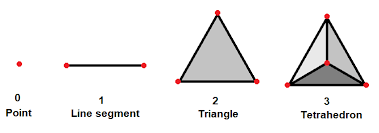
\includegraphics{resources/simplex.png}
    \caption{Simpleksi v dimenzijah 0, 1, 2 in 3. Vir: \cite{schneider_simplexes}}
    \label{fig:enter-label}
\end{figure}
\begin{comment}
    https://www.google.com/url?sa=i&url=http%3A%2F%2Fhomepages.math.uic.edu%2F~jschnei3%2FWriting%2FSimplexes&psig=AOvVaw04OUzRkF8vt7xrPuG6vtjd&ust=1714986382590000&source=images&cd=vfe&opi=89978449&ved=0CBIQjRxqFwoTCOje9KOU9oUDFQAAAAAdAAAAABAK
\end{comment}

\section{Simplicialni kompleks}
Za analizo topoloških prostorov je zelo pomembno, da jih znamo predstaviti na enostavnejši način. Za to lahko uporabljamo simplicialne komplekse, na katere lahko gledamo kot na kombinatorične opise topološkega prostora. \\
\begin{definicija}
Simplicialni kompleks \(K\) v prostoru \(R^d\) je zbirka simpleksov, tako da velja:
    \begin{enumerate}
    \item Vsako lice poljubnega simpleksa v simplicialnemu kompleksu \(K\) je tudi samo simpleks v \(K\).
    \item Naj bosta \(\sigma_1\) in \(\sigma_2\) poljubna simpleksa v \(K\). \v{C}e se sekata, potem je njun presek \(\sigma_1 \cap \sigma_2\) lice simpleksov obeh \(\sigma_1\) in \(\sigma_2\) ter je simpleks v \(K\).
\end{enumerate}
\end{definicija}

\begin{definicija}
    \textit{Geometrijski simplicialni kompleks $K$} na množici $V$ je končna množica simpleksov, ki zadoščajo naslednjima dvema pogojema:
    \begin{enumerate}
        \item Poljubno lice kateregakoli simpleksa K je simpleks v K.
        \item Presek poljubnih dveh simpleksov v K je prazna množica ali skupno lice obseh simpleksov.
    \end{enumerate}
\end{definicija}

\begin{figure}[H]
    \centering
    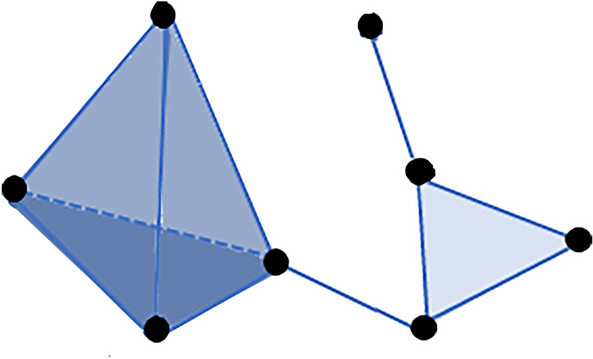
\includegraphics[width=0.8\textwidth]{resources/Simplicial-complex-eight-vertices.png}
    \caption{Simplicialni kompleks z osmimi vozlišči Vir: \cite{researchgate_simplicial_complex}}
    \label{fig:your-label}
\end{figure}
\begin{comment}
    https://www.researchgate.net/publication/358508552/figure/fig4/AS:1134810642817026@1647571349635/Simplicial-complex-An-example-of-a-simplicial-complex-composed-of-eight-vertices.png
\end{comment}

\begin{definicija}
    \textit{Abstraktni simpli\v{c}ialni kompleks} \(K\) na množici \(V\) je družina podmnožic množice \(V\), za katero velja
\[
\forall F \in K. \ G \subseteq F \implies G \in K.
\]
Množice \(F \in K\) imenujemo abstraktni simpleksi, njihovim podmnožicam \(G \subseteq F\) pa lica abstraktnega simpleksa \(F\). Dimenzijo abstraktnega simpleksa \(F\) definiramo kot \(\dim(F) = |F| - 1\). Dimenzijo abstraktnega simpli\v{c}ialnega kompleksa definiramo kot maksimalno dimenzijo njegovih simpleksov:
\[
\dim(K) = \max(\{\dim(F) \ | \ F \in K\}).
\]
\end{definicija}


\section{Gradnja simplicialnih kompleksov iz podatkov}
Simplicialne komplekse je možno zgraditi iz množice podatkov. V tem poglavju bomo opisali dva pogosto uporabljena načina. Pri tem bomo sledili \cite{10.1007/978-3-319-45378-1_1}. Privzamemo da imamo podano množico točk $X$ v metričnem prostoru $(M, d)$ in realno število $\alpha \geq 0$. Predstavili bomo dva načina, ki sta pogosto uporabljena v praksi. \cite{kun2015cech}
\begin{comment}
    https://www.jeremykun.com/2015/08/06/cech-vietoris-rips-complex/
\end{comment}

\subsection{Vietoris-Ripsov kompleks}
Prvi primer temelji na konceptu $\alpha$-soseščine. Vietoris-Ripsov kompleks $Rips_{\alpha}(\mathcal{X}) \text{ je množica simpleksov } [x_0, \ldots, x_k] \text{, tako da velja } d_{\mathcal{X}}(x_i, x_j) \leq \alpha. \text{za vse (i,j)}$. Po definiciji sledi, da je abstraktni simplicialni kompleks, v splošnem pa ne velja, da je tudi geometrični.

\subsection{Čehov kompleks}
Zelo podoben Vietoris-Ripsovem kompleksu je Čehov kompleks $C_\varepsilon$, katerega simpleksi so definirani kot množica simpleksov $[x_0, \ldots, x_k] \text{, tako da ima k + 1 zaprtih krogel} B(x_i, \alpha)$ neprazen presek.

\begin{figure}[H]
    \centering
    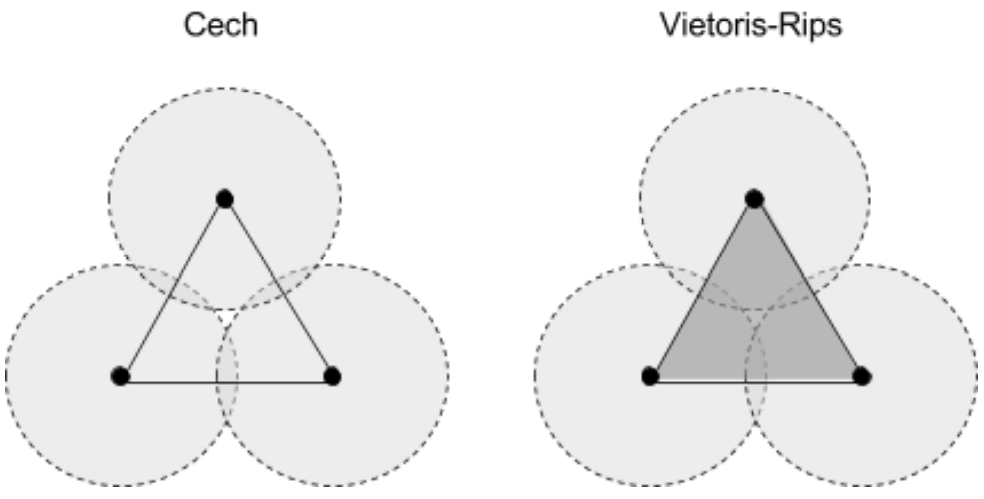
\includegraphics[width=0.7\linewidth]{resources/cech-vs-vietoris-rips-complex.png}
    \caption{Čehov in Vietoris-Ripsov kompleks. Vir: \cite{justinmath_persistent_homology}}
    \label{fig:backprop}
\end{figure}

\section{Izrek o živcu}
V tem razdelku bomo predstavili izrek o živcu, ki je osnova za Mapper algoritem, saj nam zagotavlja, da je živec, ki ga dobimo iz pokritja topološkega prostora homotopsko ekvivalenten prostoru. Izrek bomo podali brez dokaza. \cite{GuzeljBlatnik2020}

\begin{izrek}[Izrek o živcu]
Naj bo \( X \) topoološki prostor in \( \mathcal{U} = \{ U_i \}_{i \in I} \) odprto pokritje \( X \). Živec \( N(\mathcal{U}) \) pokritja \( \mathcal{U} \) je simplicialni kompleks:
\begin{itemize}
    \item Vozlišča \( N(\mathcal{U}) \) ustrezajo mnnožicam \( U_i \) v pokritju.
    \item Končna podmnožica \( \{ U_{i_0}, U_{i_1}, \ldots, U_{i_k} \} \) pokritja \( \mathcal{U} \) tvori \( k \)-simpleks v \( N(\mathcal{U}) \), če in samo če je presek \( U_{i_0} \cap U_{i_1} \cap \cdots \cap U_{i_k} \) neprazen.
\end{itemize}
Če je pokritje \( \mathcal{U} \) is \textit{dobro} (t.j., vsako končno presečišče množic v pokritju je bodisi prazno bodisi kontraktibilno), potem je topološki prostor \( X \) homotopsko ekvivalenten živcu \( N(\mathcal{U}) \). Z drugimi besedami,
\[ X \simeq N(\mathcal{U}). \]
\end{izrek}